\documentclass[border=15pt, tikz]{standalone}
\usepackage[T1]{fontenc}
\usepackage[utf8]{inputenc}
\usepackage{tikz}
\usetikzlibrary{positioning, arrows.meta, decorations.pathreplacing, calc, fit}
\definecolor{clrattention}{HTML}{45B7D1}
\definecolor{clrattention_alt}{HTML}{96E6F0}
\definecolor{clrffn}{HTML}{F97068}
\definecolor{clrnorm}{HTML}{FFD93D}
\definecolor{clrembed}{HTML}{6BCB77}
\definecolor{clrresidual}{HTML}{4D96FF}
\definecolor{clroutput}{HTML}{C084FC}
\definecolor{clrspectral}{HTML}{22D3EE}
\definecolor{clrphysics}{HTML}{FB923C}
\definecolor{clrborder}{HTML}{334155}
\definecolor{clrtext}{HTML}{1E293B}
\definecolor{clrgroup_frame}{HTML}{94A3B8}
\definecolor{clrgroup_fill}{HTML}{F1F5F9}
\begin{document}
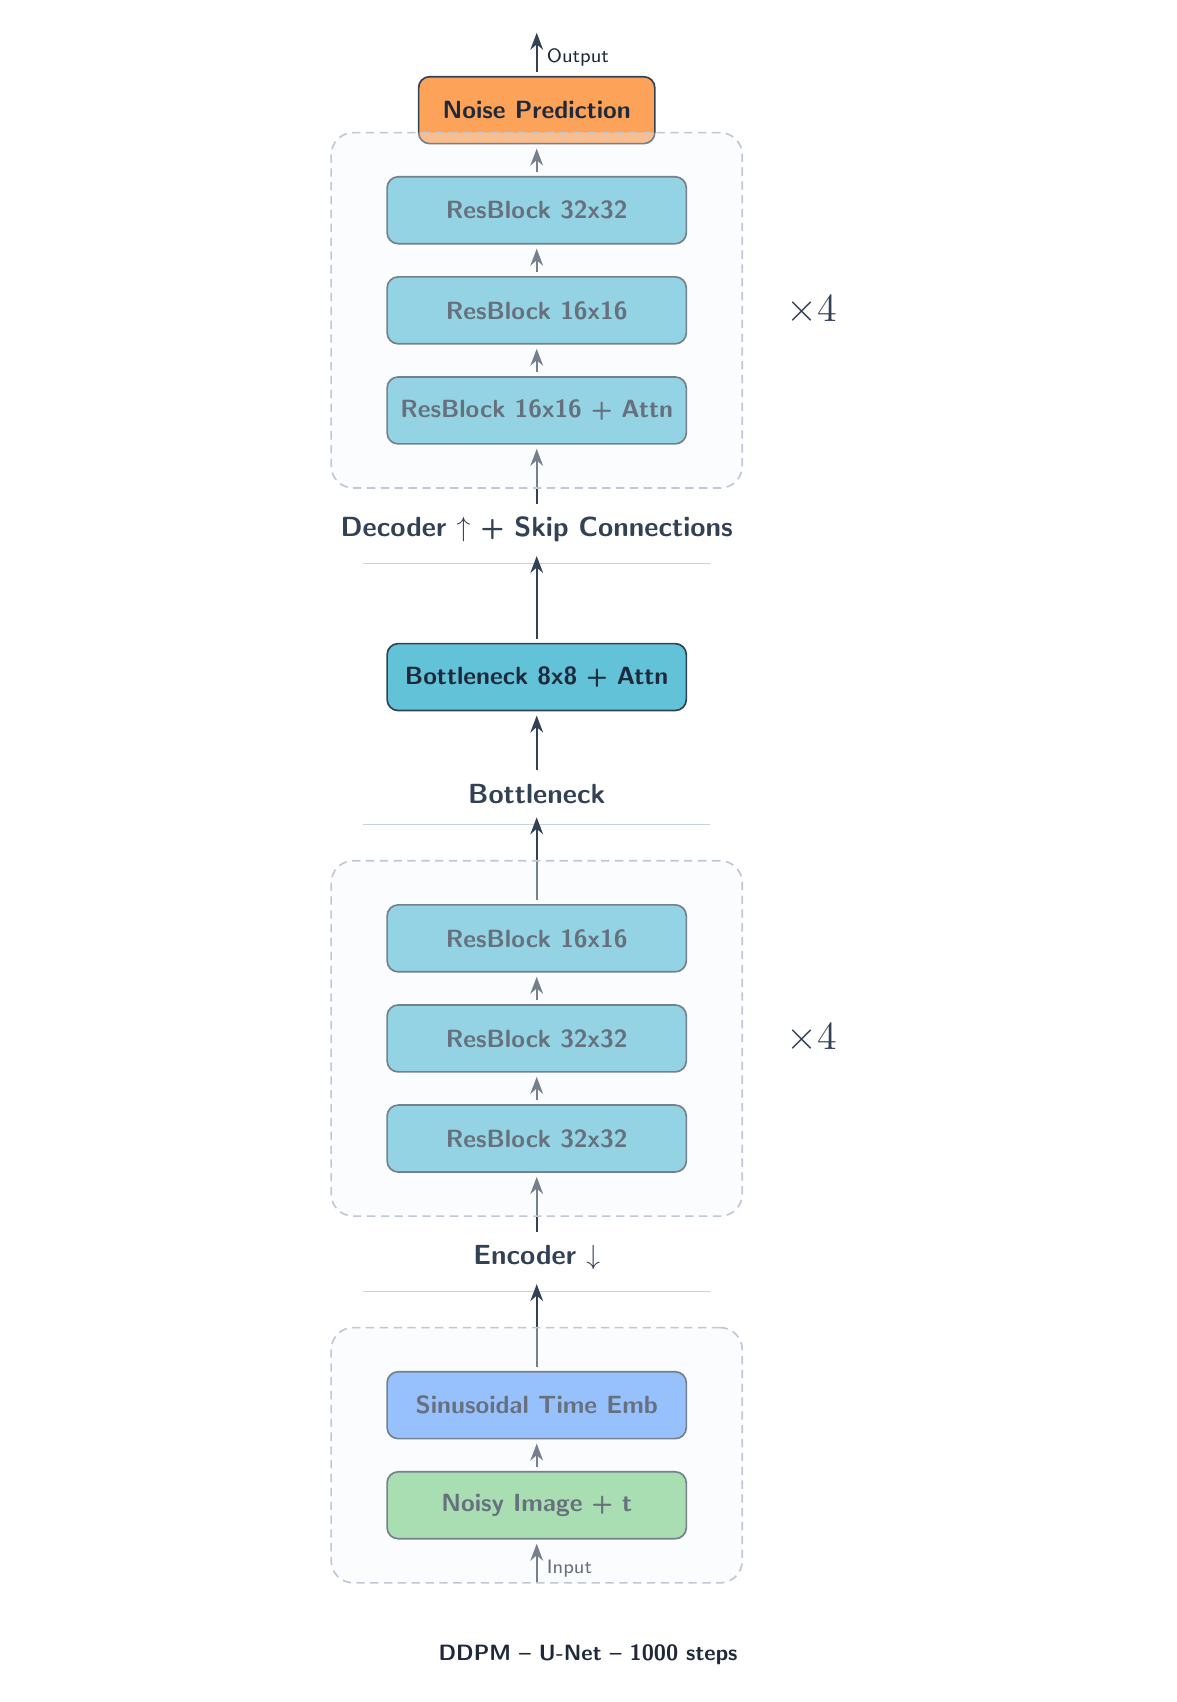
\begin{tikzpicture}[
    >=Stealth,
    every node/.style={font=\sffamily},
    block/.style={draw=clrborder, rounded corners=4pt, minimum width=3.8cm,
                  minimum height=0.85cm, font=\sffamily\small\bfseries,
                  text=clrtext, line width=0.6pt},
    arrow/.style={->, thick, color=clrborder, line width=0.7pt, shorten >=1.5pt, shorten <=1.5pt},
    skiparrow/.style={->, thick, color=clrresidual, line width=0.8pt, rounded corners=4pt, shorten >=1.5pt},
    label/.style={font=\sffamily\scriptsize, text=clrtext},
    subtitle/.style={font=\sffamily\footnotesize, text=clrtext},
]
\node[block, fill=clrembed!85, minimum width=3.8cm, minimum height=0.85cm, text=clrtext] (n_1) at (0,0) {Noisy Image + t};
\node[block, fill=clrresidual!85, minimum width=3.8cm, minimum height=0.85cm, text=clrtext, above=0.4cm of n_1] (n_2) {Sinusoidal Time Emb};
\node[inner sep=0, minimum height=0, above=1.0cm of n_2] (n_3_rule) {};
\draw[color=clrgroup_frame!50, line width=0.4pt] ([xshift=-2.2cm]n_3_rule.center) -- ([xshift=2.2cm]n_3_rule.center);
\node[above=4pt of n_3_rule, font=\sffamily\normalsize\bfseries, text=clrborder] (n_3) {Encoder $\downarrow$};
\node[block, fill=clrattention!85, minimum width=3.8cm, minimum height=0.85cm, text=clrtext, above=0.8cm of n_3] (n_4) {ResBlock 32x32};
\node[block, fill=clrattention!85, minimum width=3.8cm, minimum height=0.85cm, text=clrtext, above=0.4cm of n_4] (n_5) {ResBlock 32x32};
\node[block, fill=clrattention!85, minimum width=3.8cm, minimum height=0.85cm, text=clrtext, above=0.4cm of n_5] (n_6) {ResBlock 16x16};
\node[inner sep=0, minimum height=0, above=1.0cm of n_6] (n_7_rule) {};
\draw[color=clrgroup_frame!50, line width=0.4pt] ([xshift=-2.2cm]n_7_rule.center) -- ([xshift=2.2cm]n_7_rule.center);
\node[above=4pt of n_7_rule, font=\sffamily\normalsize\bfseries, text=clrborder] (n_7) {Bottleneck};
\node[block, fill=clrattention!85, minimum width=3.8cm, minimum height=0.85cm, text=clrtext, above=0.8cm of n_7] (n_8) {Bottleneck 8x8 + Attn};
\node[inner sep=0, minimum height=0, above=1.0cm of n_8] (n_9_rule) {};
\draw[color=clrgroup_frame!50, line width=0.4pt] ([xshift=-2.2cm]n_9_rule.center) -- ([xshift=2.2cm]n_9_rule.center);
\node[above=4pt of n_9_rule, font=\sffamily\normalsize\bfseries, text=clrborder] (n_9) {Decoder $\uparrow$ + Skip Connections};
\node[block, fill=clrattention!85, minimum width=3.8cm, minimum height=0.85cm, text=clrtext, above=0.8cm of n_9] (n_10) {ResBlock 16x16 + Attn};
\node[block, fill=clrattention!85, minimum width=3.8cm, minimum height=0.85cm, text=clrtext, above=0.4cm of n_10] (n_11) {ResBlock 16x16};
\node[block, fill=clrattention!85, minimum width=3.8cm, minimum height=0.85cm, text=clrtext, above=0.4cm of n_11] (n_12) {ResBlock 32x32};
\node[block, fill=clrphysics!85, minimum width=3.0cm, minimum height=0.85cm, text=clrtext, above=0.4cm of n_12] (n_13) {Noise Prediction};
\draw[arrow] (n_1.north) -- (n_2.south);
\draw[arrow] (n_2.north) -- (n_3.south);
\draw[arrow] (n_3.north) -- (n_4.south);
\draw[arrow] (n_4.north) -- (n_5.south);
\draw[arrow] (n_5.north) -- (n_6.south);
\draw[arrow] (n_6.north) -- (n_7.south);
\draw[arrow] (n_7.north) -- (n_8.south);
\draw[arrow] (n_8.north) -- (n_9.south);
\draw[arrow] (n_9.north) -- (n_10.south);
\draw[arrow] (n_10.north) -- (n_11.south);
\draw[arrow] (n_11.north) -- (n_12.south);
\draw[arrow] (n_12.north) -- (n_13.south);
\draw[arrow] ([yshift=-0.6cm]n_1.south) -- node[right, yshift=-2pt, font=\sffamily\scriptsize, text=clrtext] {Input} (n_1.south);
\draw[arrow] (n_13.north) -- node[right, yshift=-2pt, font=\sffamily\scriptsize, text=clrtext] {Output} ([yshift=0.6cm]n_13.north);
\node[draw=clrgroup_frame!60, rounded corners=8pt, densely dashed, line width=0.6pt, fill=clrgroup_fill, fill opacity=0.35, inner ysep=0.55cm, inner xsep=0.7cm, fit=(n_1) (n_2)] (g_0) {};
\node[draw=clrgroup_frame!60, rounded corners=8pt, densely dashed, line width=0.6pt, fill=clrgroup_fill, fill opacity=0.35, inner ysep=0.55cm, inner xsep=0.7cm, fit=(n_4) (n_5) (n_6)] (g_1) {};
\node[right=12pt of g_1.east, anchor=west, font=\sffamily\Large\bfseries, text=clrborder] (g_1_badge) {$\times4$};
\node[draw=clrgroup_frame!60, rounded corners=8pt, densely dashed, line width=0.6pt, fill=clrgroup_fill, fill opacity=0.35, inner ysep=0.55cm, inner xsep=0.7cm, fit=(n_10) (n_11) (n_12)] (g_2) {};
\node[right=12pt of g_2.east, anchor=west, font=\sffamily\Large\bfseries, text=clrborder] (g_2_badge) {$\times4$};
\node[below=0.6cm of current bounding box.south, subtitle, text width=14cm, align=center] {\textbf{DDPM -- U-Net -- 1000 steps}};
\end{tikzpicture}
\end{document}
